\section*{Appendix A: Intuition on Convergence}

  Unlike convergence of numbers, which is well-defined with respect to some metric or topology, there are many types of convergence of random variables. We must always specify which convergence when talking about them. Remember that a random variable $X$ is just a function from $\Omega$ to $\mathbb{R}$, so we can talk about pointwise convergence. That is, given a sequence of random variables $\{X_n\}$ and some $\omega \in \Omega$, the sequence 
  \begin{equation}
    X_1(\omega), X_2 (\omega), X_3(\omega), \ldots
  \end{equation}
  is simply a sequence of real numbers. If this sequence converges to the real number $X(\omega)$, then $X_n$ converges to $X$ at $\omega$. If this occurs for all $\omega \in \Omega$, then we have sure convergence, and if this happens for an event (a $\mathcal{F}$-measurable subset of $\Omega$) with probability $1$, then we have almost sure convergence. 

  \begin{definition}[Sure Convergence of RVs]
    The sequence of random variables $\{ X_n\}_{n \in \mathbb{N}}$ is said to \textbf{converge pointwise} or \textbf{converge surely} to $X$ if 
    \begin{equation}
      X_n (\omega) \rightarrow X (\omega)
    \end{equation}
    for every $\omega \in \Omega$. That is, we can choose \textit{any} $\omega \in \Omega$, and the realized sequence $X_1 (\omega), X_2 (\omega), \ldots$ will always converge to $X(\omega)$. 
  \end{definition}

  But this definition is too strong of a form of convergence, since in probability we don't care about values over sets of measure $0$. That is, if we have two probability distributions that differ from each other on a set of measure $0$, then they can be considered essentially the same probability distribution. 

  \begin{definition}[Almost Sure Convergence of RVs]
    The sequence of random variables $\{ X_n\}_{n \in \mathbb{N}}$ is said to \textbf{converge almost surely} or \textbf{converge with probability 1} to $X$ if $X_n (\omega) \rightarrow X (\omega)$ on a subset of probability $1$. That is, 
    \begin{equation}
      \mathbb{P} \big( \{ \omega \in \Omega \mid \lim_{n \rightarrow \infty} X_n (\omega) = X(\omega) \} \big) = 1
    \end{equation}
    Crudely put, we just have to look at each $\omega \in \Omega$, see if $X_n (\omega)$ converges to $X(\omega)$ as $n \rightarrow \infty$, and determine if the set of all $\omega$'s that satisfy this have probability $1$. In other words, let us have some experiment with outcome space $\Omega$. With probability $1$, some $\omega \in \Omega$ will be realized, which will realize the sequence of realized random variables
    \begin{equation}
      X_1 (\omega), X_2 (\omega), X_3 (\omega), \ldots
    \end{equation}
    that will converge to $X(\omega)$. 
  \end{definition}

  \begin{definition}[Convergence in Probability]
    The sequence of random variables $\{ X_i\}_{i \in \mathbb{N}}$ is said to \textbf{converge to $X$ in probability} if for all $\epsilon > 0$, 
    \begin{equation}
      \lim_{n \rightarrow \infty} \mathbb{P} \big( |X_n - X| > \epsilon \big) = 0
    \end{equation}
    To understand what this means, fix an $\epsilon > 0$. Then, $X_1$ may be very far from $X$, meaning that the event $|X_1 - X| > \epsilon$, i.e. the set of all $\omega \in \Omega$ satisfying $|X_1(\omega) - X (\omega)| > \epsilon$ may be a larger portion of $\Omega$. Now, as we increase $n$, this event will become smaller (in the way that it's probability decreases) until it reaches $0$. 
    \begin{center}
      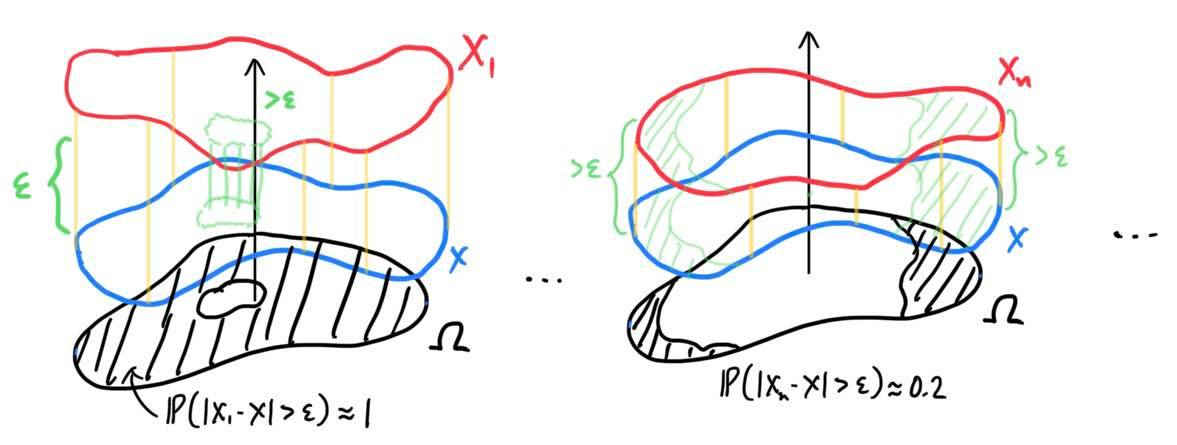
\includegraphics[scale=0.3]{img/convergence_in_probability.jpg}
    \end{center}
  \end{definition}

  \begin{example}
    Given $X_n \sim \mathrm{Exponential}(n)$ with $f_{X_n} (x) = n e^{-nx}$, we show that the sequence converges in probability to the $0$ random variable. Given $\epsilon > 0$, we have 
    \begin{align*}
      \lim_{n \rightarrow \infty} \mathbb{P}(|X_n - 0| > \epsilon) & = \lim_{n \rightarrow \infty} \mathbb{P}(X_n > \epsilon \cup X_n < -\epsilon) \\
      & = \lim_{n \rightarrow \infty} \mathbb{P}(X_n > \epsilon) \\
      & = \lim_{n \rightarrow \infty} \int_\epsilon^\infty n e^{-nx} \,dx \\
      & = \lim_{n \rightarrow \infty} e^{-n \epsilon} = 0
    \end{align*}
    We can imagine this since given any small $\epsilon > 0$, we can see that increasing $n$ results in the distribution of $X_n$ to decrease at a faster rate, and thus a bigger portion of the distribution would lie within $\epsilon$ of the $0$ random variable. 
    \begin{center}
      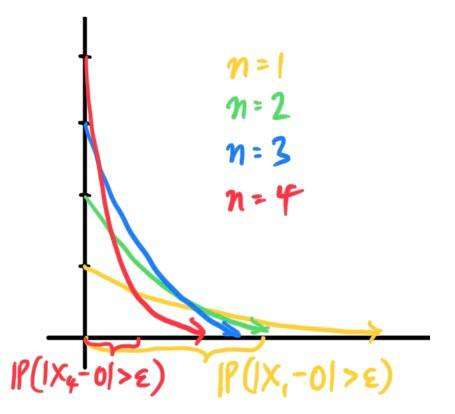
\includegraphics[scale=0.3]{img/convergence_in_prob_exponential.jpg}
    \end{center}
  \end{example}

\subsection{Convergence in Probability vs Almost Surely} 

  Convergence almost surely and convergence with probability are very different. Almost sure convergence has the limit inside the probability, which indicates that we are talking about convergence of a sequence of random variables. On the other hand, convergence in probability has the limit on the outside, which talks about convergence of a sequence of probabilities. But a key point is that almost sure convergence implies convergence in probability. It happens so because there could exist a subset of small probability in $\Omega$ where the $X_n$'s and $X$ need not be close, but the probabilities of them deviating over whole $\Omega$ is small. 

  \begin{example}[C. in Probability $\centernot\implies$ C. Almost Surely]
    Consider the interval $\Omega = [0, 1]$ and the subsets $A_1 = [0, 0.1], A_2 = [0.1, 0.2], \ldots$, such that at $A_{10} = [0.9, 1.0]$, the size with halve and will go to the left boundary, $A_{11} = [0, 0.05], \ldots$. Then, the sequence of indicator random variables 
    \begin{equation}
      X_n \coloneqq 1_{A_n}
    \end{equation}
    looks like it's converging to the $0$ random variable. Indeed, $X_n \xrightarrow{i.p.} 0$ since the probability that $X_n$ deviates from $0$ by more than some small $\epsilon$ is simply the measure of $A_n$ itself, which decreases to $0$. That is, given some small $\epsilon > 0$, we have 
    \begin{equation}
      \lim_{n \rightarrow \infty} \mathbb{P} (|X_n - 0| > \epsilon) = \lim_{n \rightarrow \infty} \mathbb{P}(1_{A_n} > \epsilon ) = \lim_{n \rightarrow \infty} \mathbb{P}(A_n) = 0
    \end{equation}
    Now let's show that this doesn't converge almost surely. For \textit{any} outcome $\omega \in \Omega$, the sequence of random variables $X_1(\omega), X_2(\omega), \ldots$ will hit these intervals $A_n$ infinitely many times and will not converge to $0$, since there will always be a $1$ down the sequence. They will occur with decreasing frequency but they will always occur. Therefore, with probability $1$, whatever realized sequence will not converge to the $0$ random variable. 
  \end{example}

  Here is another standard counterexample. 

  \begin{example}[C. in Probability $\centernot\implies$ C. Almost Surely]
    Let us take the sequence $X_1, X_2, \ldots$ of independent random variables where $X_n \sim \mathrm{Bernoulli}(1/n)$. That is, 
    \begin{equation}
      \mathbb{P}(X_n = 1) = \frac{1}{n} \text{ and } \mathbb{P}(X_n = 0) = 1 - \frac{1}{n}
    \end{equation}
    So, as $n$ gets large we expect $X_n$ to realize values of $0$ more and more. Showing that $X_n \xrightarrow{i.p.} 0$ is easy, since we can compute for any $\epsilon > 0$
    \begin{align*}
      \lim_{n \rightarrow \infty} \mathbb{P}(|X_n - 0| > \epsilon) & = \lim_{n \rightarrow \infty} \mathbb{P}(|X_n| > \epsilon) \\
      & = \lim_{n \rightarrow \infty} \mathbb{P}(X_n = 1) \\
      & = \lim_{n \rightarrow \infty} \frac{1}{n} = 0
    \end{align*}
    We want to show that this does not converge almost surely to $0$, i.e. there is some set of nonzero measure such that for some $\omega$ in that set, the sequence $X_1 (\omega), X_2(\omega), \ldots$ does not converge to $0$. This can be hard to see at first, but the fact that we have independence and the terms are $\frac{1}{n}$ hints at the Borel-Cantelli lemma. Let $A_n$ be the event that $\{X_n = 1\}$ (i.e. the preimage of the singleton set under $X_n$: $X_n^{-1} ( \{1\})$). Then, the $A_n$'s are independent, and 
    \begin{equation}
      \sum_{n=1}^\infty \mathbb{P}(A_n) = +\infty
    \end{equation}
    By the Borel-Cantelli lemma 2, this implies that almost surely infinitely many $A_n$'s will occur. That is, we can choose as large of an $n$ as we like, go down the sequence until we look at $X_n, X_{n+1}, \ldots$, and we are guaranteed with probability $1$ that at least one of the $X_i$'s after $n$ will realize a $1$. This means that in every realization of $X_1, X_2, \ldots$, we will get a sequence of $0$s and $1$s, but since BCL states that no matter how far down the road you will always get at least another $1$, this sequence does not converge to $0$.  
  \end{example}

  The commonality between these two examples is that sequence of random variables satisfies convergence in probability as follows: As $n$ increases, $X_n$ is more and more likely to be near $X$ (in the way that $|X_n - X| < \epsilon$ for some $\epsilon > 0$), ultimately satisfying this closeness property with probability $1$ as $n \rightarrow \infty$. For example, we could have 
  \begin{align*}
    \mathbb{P}(|X_1 - X| > \epsilon) & = 1 \\
    \mathbb{P}(|X_2 - X| > \epsilon) & = 1/2 \\
    \mathbb{P}(|X_3 - X| > \epsilon) & = 1/3 \\
    \ldots & = \ldots 
  \end{align*}
  This definitely satisfies convergence in probability, but this leaves open the possibility that $\mathbb{P}(|X_n - X| > \epsilon)$ an infinite number of times, although at infrequent intervals. Therefore, when looking at the sequence 
  \begin{equation}
    X_1, X_2, X_3, \ldots
  \end{equation}
  each random variable \textit{individually} may have less chance of being more than $\epsilon$ away from $X$, but since there is an infinite number of them in the sequence, the sequence \textit{in totality} may contain an infinite number of cases where $|X_n - X| > \epsilon$. Convergence almost surely tells us that we are \textit{guaranteed} (with probability $1$) that this sequence will converge to $X$. That is, we can specify an $N \in \mathbb{N}$ such that $|X_n - X| < \epsilon$ for all $n > N$. 

  Let us define some $\epsilon > 0$ and consider a sequence of random variables $\{X_n\}_{n \in \mathbb{N}}$. Given some outcome $\omega \in \Omega$, we will consider it a \textit{success} if $|X_n(\omega) - X(\omega)| < \epsilon$ and \textit{failure} if not. Then, convergence in probability tells us that the probability of failure goes to $0$ as $n$ goes to infinity and therefore we get better and better estimates of $X$. Convergence almost surely is a bit stronger and says that the total number of failures is \textit{finite}. That is, after a certain point $N$, the random variable $X_n$ will \textit{always} estimate $X$ within an error of $\epsilon$ (i.e. such that $|X_n - X| < \epsilon$). But since you don't know when you've exhausted all failures, there is not much of a difference from a practical point of view. 

\subsection{Complete Convergence}

  When proving almost sure convergence, we'd ideally just look at all the $\omega \in \Omega$ where $X_n (\omega) \rightarrow X(\omega)$, and if this set has probability measure $1$, then we are done. But this is not very practical, so we use the following theorem, which gives a sufficient condition for $X_n \xrightarrow{a.s.} X$. 

  \begin{theorem}
    If for all $\epsilon > 0$, 
    \begin{equation}
      \sum_{n=1}^\infty \mathbb{P}(|X_n - X| > \epsilon ) < \infty
    \end{equation}
    then $X_n \xrightarrow{a.s.} X$. This condition is a bit stronger, since not only are we saying that $\mathbb{P}(|X_n - X| > \epsilon)$ tends to $0$ as $n \rightarrow \infty$, but that it goes down fast enough to keep the series convergent. 
  \end{theorem}
  \begin{proof}
    Let the event that $|X_n - X| > \epsilon$ be denoted $A_n (\epsilon)$ (i.e. the preimage of $(\epsilon, \infty)$ under the map $|X_n - X|$, which is a $\mathcal{F}$-measurable set). Since the sum of their probabilities is finite, by the Borel-Cantelli lemma 1, finitely many $A_n(\epsilon)$'s will occur with probability $1$. This means that for any $\epsilon > 0$, $|X_n - X| \leq \epsilon$ for all large enough $n$, meaning that it converges to $0$. 
  \end{proof}

